
\chapter{Monte Carlo Generation and Reconstruction}

The Monte Carlo (MC) for this analysis was generated using the RAPGAP software package. RAPGAP is a generator for eletron-proton MC. The structure functions measured at HERA are used to model a variety of diffractive processes. Each event has a characteristic energy for the virtual photon exchanged by the electron and proton. This photon energy is used to reweigh the MC to model the energy distribution of the Weizacker Williams photon flux. 

\begin{equation}
w(E) = \frac{\mathrm{d} N^{eff}_\gamma}{\mathrm{d} E} / \frac{\mathrm{d} N^{RAPGAP}_\gamma }{\mathrm{d} E}
\end{equation}
$\mathrm{d} N^{RAPGAP}_\gamma / \mathrm{d} E$ is obtained by fitting the formula for the total electron-proton cross-section, $\sigma_{\gamma p}$ to the RAPGAP MC's energy distribution. 

\begin{figure}[h!]
\begin{centering}
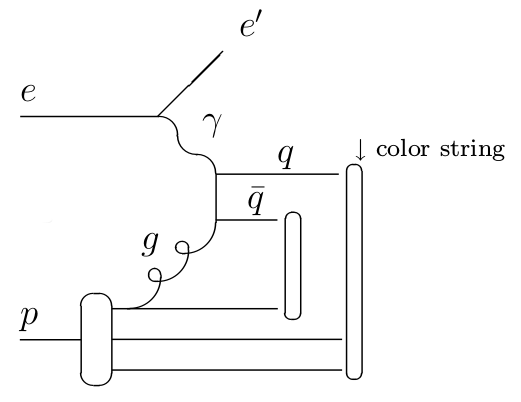
\includegraphics[width=4in]{Appendix1/importfigs/rapgap_diagram.png}
\par\end{centering}
\caption{RAPGAP process: boson-gluon fusion. \label{fig:rapgap_diagram}}
\end{figure}

\begin{equation}
\frac{\mathrm{d}^2 \sigma_{ep} }{\mathrm{d} y \; \mathrm{d} Q^2} = \frac{\alpha}{2 \pi Q^2}\left ( \frac{1+(1-y)^2)}{y} - \frac{2(1-y)}{y}\cdot \frac{Q^2_{min}}{Q^2} \right )\cdot \sigma^{tot}_{\gamma^*p}(W_{\gamma^*p}),
\end{equation}
where 
\begin{equation}
Q^2_{min}\approx \frac{m_e^2 \; y^2}{1-y}.
\end{equation}
In this context, $y$ is the energy fraction carried away from the electron by the mediating virtual photon, $Q^2$ is the photon virtuality, $m_e$ is the electron mass, $\sigma^{tot}_{\gamma^*p}(W_{\gamma^*p})$ is the total photon-proton cross section, and $W_{\gamma^*p}$ is the center of mass energy of the photon-proton collision. 

\begin{figure}%
    \centering
    \subfloat[label 1]{{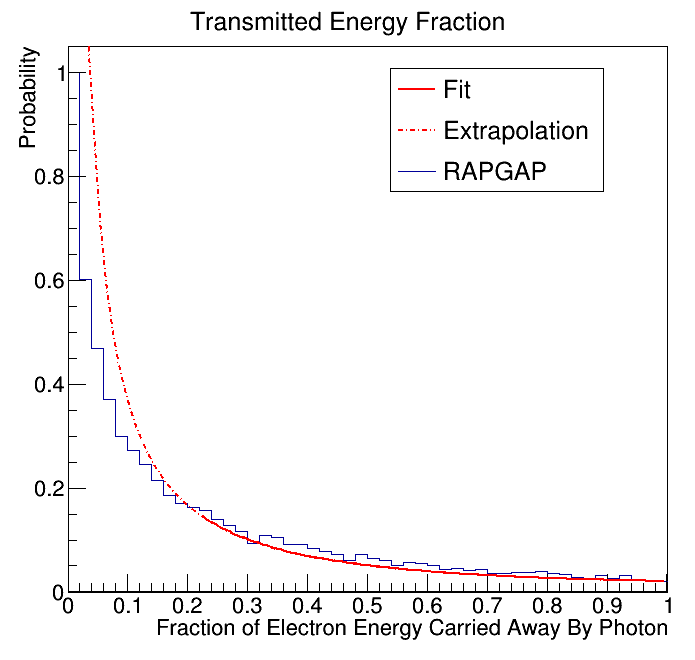
\includegraphics[width=7.cm]{Appendix1/importfigs/before_fit.png} }}%
    \qquad
    \subfloat[label 2]{{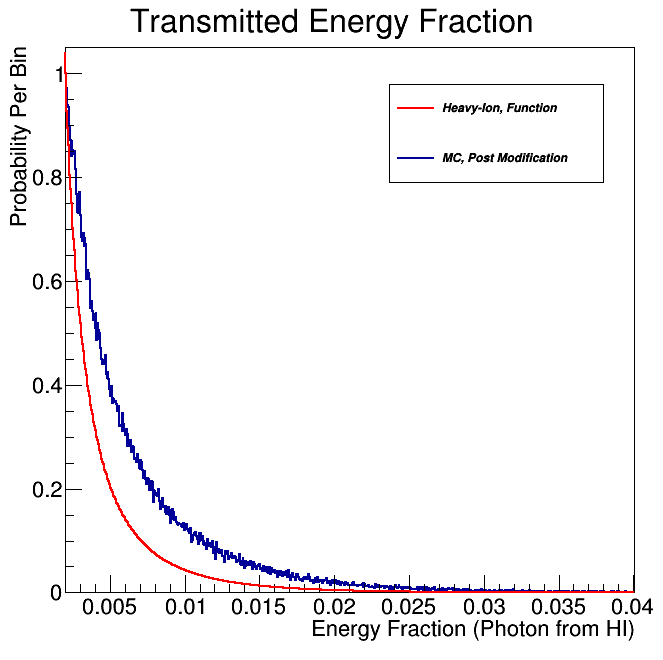
\includegraphics[width=7.cm]{Appendix1/importfigs/after_fit.png} }}%
    \caption{Left: Energy Distribution Before Fitting, Right: Energy Distribution After Fitting}%
    \label{fig:patKennyPlots}%
\end{figure}
